% GEOMIRA export: TikZ. One unit is 25.657718bp (34.210291 px on screen).
% Needs \usepackage{tikz} and \usepackage{amssymb}.
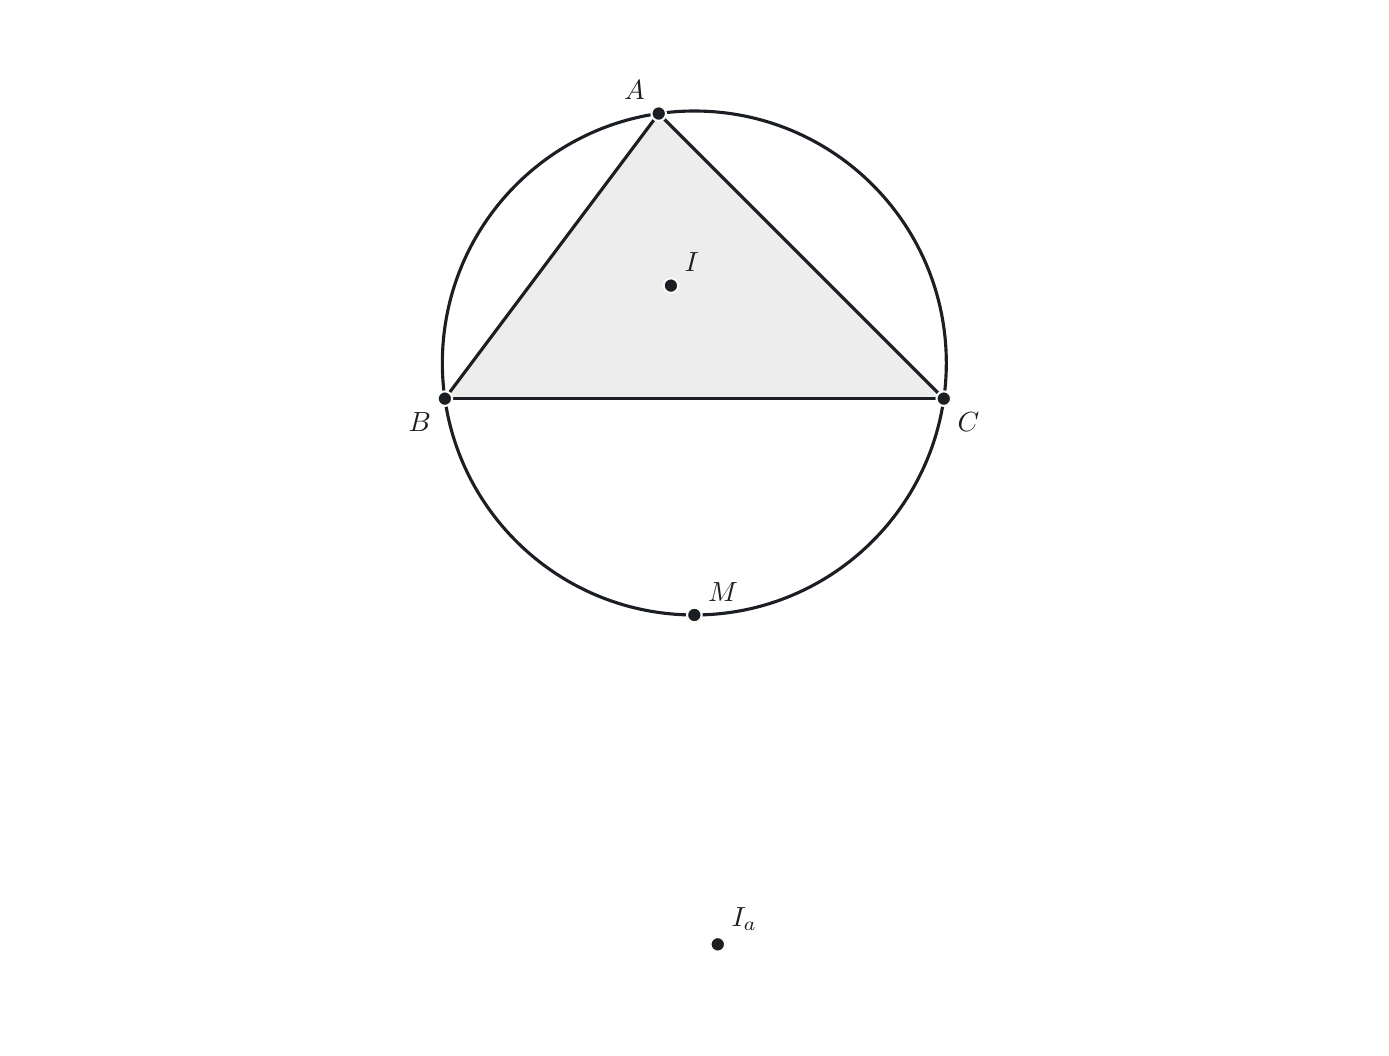
\begin{tikzpicture}[x=25.657718bp, y=25.657718bp, line cap=round, line join=round]
\definecolor{gmc0}{HTML}{1B1F24}
\definecolor{gmc1}{HTML}{FBFBF8}
\clip (-7.8539,-8.8261) rectangle (10.8539,5.2048);
% abc
\fill[gmc0, fill opacity=0.08] (1,4) -- (-2,0) -- (5,0) -- cycle;
\draw[gmc0, line width=1.125bp] (1,4) -- (-2,0);
\draw[gmc0, line width=1.125bp] (-2,0) -- (5,0);
\draw[gmc0, line width=1.125bp] (5,0) -- (1,4);
% ω
\draw[gmc0, line width=1.125bp] (5.0355,0.5) arc[start angle=0, end angle=360, radius=3.53553];
% A
\filldraw[fill=gmc0, draw=gmc1, line width=0.75bp] (1,4) circle[radius=2.625bp];
% B
\filldraw[fill=gmc0, draw=gmc1, line width=0.75bp] (-2,0) circle[radius=2.625bp];
% C
\filldraw[fill=gmc0, draw=gmc1, line width=0.75bp] (5,0) circle[radius=2.625bp];
% I
\filldraw[fill=gmc0, draw=gmc1, line width=0.75bp] (1.1716,1.5858) circle[radius=2.625bp];
% I_a
\filldraw[fill=gmc0, draw=gmc1, line width=0.75bp] (1.8284,-7.6569) circle[radius=2.625bp];
% M
\filldraw[fill=gmc0, draw=gmc1, line width=0.75bp] (1.5,-3.0355) circle[radius=2.625bp];
\node[anchor=south east, inner sep=0pt, text=gmc0] at (0.814,4.186) {$A$}; % label of A
\node[anchor=north east, inner sep=0pt, text=gmc0] at (-2.186,-0.186) {$B$}; % label of B
\node[anchor=north west, inner sep=0pt, text=gmc0] at (5.186,-0.186) {$C$}; % label of C
\node[anchor=south west, inner sep=0pt, text=gmc0] at (1.3576,1.7718) {$I$}; % label of I
\node[anchor=south west, inner sep=0pt, text=gmc0] at (2.0145,-7.4708) {$I_{a}$}; % label of I_a
\node[anchor=south west, inner sep=0pt, text=gmc0] at (1.686,-2.8495) {$M$}; % label of M
\end{tikzpicture}
